\section{Generalized Cross Correlation}

As depict in \ref{sec:cc}, the \ac{CC} can bring some error sources in the context of
incorrect delay results and inaccuracy.
Improvements were done in research by introducing prefilters for the signals
which is equal to general frequency weighting as stated in \cite{K_C_GCC}.
\begin{figure}[ht]
	\centering
		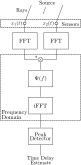
\includegraphics[width=0.35\columnwidth]{figures/GCC_weight}
	\caption{Generalized cross correlation for time delay estimation}
    \label{fig:02_GCC}
\end{figure}
With certain weightings $H_i(f)$ prior to the \ac{CC}, the peak detection
can be rectified by improving the relation between peak and noise or
enhancing the accuracy \cite{H_B_GCC}.
Figure \ref{fig:02_GCC} illustrates the process of a \ac{GCC} with both filters combined as
$\Psi(f) = H_1^*(f)H_2$. The figure in \ref{appendix:a1_alternativeGcc} represents the
\ac{GCC} with $H_i(f)$.
After transforming the signals $x_i(f)$ into frequency domain, the cross correlated
signals are multiplied with the weighting $\Psi(f)$ and transformed back into time domain.
The following steps are similar to the \ac{CC}.
Thus, the \ac{GCC} is declared as
\bal
    R^{(g)}_{x_1x_2}(t) = \int^{+\infty}_{-\infty}\Psi(f)G_{x_1x_2}(f)e^{j2\pi ft} df.
\eal
\label{eq:02_gcc}
Written-out it is visible how the choice of $\Psi(f)$ impacts the individual segments of \ref{eq:02_Gx1x2}
as
\unsure[]{Why is there an indent?}
\bal
    R^{(g)}_{x_1x_2}(f) &= \mathcal{F}^{-1}[\Psi(f) \alpha \phi_s(f) e^{-j2\pi fD}] \nonumber \\
    &+ \mathcal{F}^{-1}[\Psi(f) \phi_n(f)] + \mathcal{F}^{-1}[\Psi(f) \phi_c(f)].
\eal
\label{eq:02_gcc_long}
Several variants of the weighting were designed by various researchers with different criteria.
The effect of the most common filters will be shortly pointed out in the following.
%_______________________________________________________________________________________________________________
\subsection{The Phase Transform (PHAT)}
The \ac{PHAT} weighting is known as
\bal
    \Psi^{(P)}(f) = \frac{1}{|G_{x_1x_2}(f)|}.
\eal
For the ideal case that $\phi_n$ and $\phi_c$ are nonexistent, the the \ac{GCC} results in
\bal
    R^{(p)}_{x_1x_2}(t) = \mathcal{F}^{-1}[\frac{\alpha |S(f)|^2 e^{-j2\pi fD}}{|G_{x_1x_2}(f)|}] = \delta(t-D)
\eal
because $|G_{x_1x_2}(f)| = \alpha |S(f)|^2$.
This filter is used regularly in research, because the peak is not spread by the signal spectrum what gives
a high accuracy.

%- whistle frequency between 2000Hz and 4000Hz (low-pass)\\
%- thus, the peaks of the cross-correlation are wide\\